\documentclass[11pt]{article}

% ACL final-format template package. The course requested the ACL/Overleaf
% structure; the submission source includes acl.sty, acl_natbib.bst, and custom.bib.
\usepackage{acl}
\usepackage[T1]{fontenc}
\usepackage[utf8]{inputenc}
\usepackage{microtype}
\usepackage{graphicx}
\usepackage{booktabs}
\usepackage{array}
\usepackage{amsmath}
\usepackage{enumitem}
\usepackage{xurl}
\urlstyle{same}
\setlist[itemize]{leftmargin=1.2em,itemsep=1pt,topsep=2pt}
\newcommand{\lcb}{LiveCodeBench}
\newcommand{\passone}{pass@1}

\title{Survey: Measuring Algorithmic Progress in Modern LLMs on Competitive Programming via LiveCodeBench}

\author{An Quoc Nguyen \\
  University of South Florida \\
  \texttt{anguyen56@usf.edu}}

\begin{document}
\maketitle
\begin{abstract}
Modern language models have improved quickly on code generation benchmarks, but static tests such as HumanEval and MBPP can be distorted by benchmark saturation and training-data contamination. This report surveys algorithmic progress in large language models (LLMs) using \lcb{}, a continuously updated competitive-programming benchmark with time-stamped tasks. The empirical component is a controlled release\_v5 run on 279 post-August-2024 problems comparing Claude Sonnet 4.6, Qwen2.5-Coder-7B-Instruct, and DeepSeek-Coder-V2-Lite-Instruct on code generation and self-repair. Claude Sonnet 4.6 solves 66.3\% of problems in code generation and 69.9\% after self-repair, while Qwen2.5-Coder and DeepSeek-Coder-V2-Lite solve 17.6\% and 17.6\% initially. Difficulty stratification shows the bottleneck: Claude reaches 97.0\% on Easy problems but 37.4\% on Hard problems, and both open models fall to 3.3\% on Hard. Self-repair gives small gains: +3.6 points for Claude, +1.4 for DeepSeek, and no measured gain for Qwen. The pattern is clear: recent LLM progress is real, but it is uneven, and the hardest remaining work is multi-step algorithm design and debugging rather than basic syntax generation.
\end{abstract}

\section{Introduction}
Large language models are now common tools for software engineering, competitive programming assistance, and AI agent workflows. Coding performance is often summarized by a single aggregate number on a benchmark, yet that number can hide the difference between memorized solutions, shallow pattern completion, and algorithmic reasoning. The distinction shows up sharply in competitive programming because problems are intentionally designed to require nontrivial choices: dynamic programming recurrences, graph traversals, greedy exchange arguments, bitmask state compression, binary search over answers, segment trees, and careful boundary handling. A model that writes plausible Python syntax may still fail if it chooses an $O(n^2)$ method for an input size requiring $O(n \log n)$, misses a proof obligation, or cannot adapt after a failing hidden test.

Older code benchmarks are no longer enough on their own. HumanEval evaluates Python function completion and helped standardize pass-rate reporting \citep{chen2021codex}. MBPP similarly evaluates short programming tasks \citep{austin2021program}. These datasets remain useful for comparability, but they are small, public, and heavily reused. Once a benchmark becomes part of public evaluation culture, future models may see near-duplicate solutions during pretraining or instruction tuning. A high score can reflect contamination or benchmark-specific overfitting rather than the ability to solve new programming tasks. Competition-level datasets such as CodeContests and AlphaCode-oriented evaluations moved toward more demanding algorithmic problems \citep{li2022competition}, and reasoning-oriented tests such as CRUXEval separated code execution from code writing \citep{gu2024cruxeval}. What is still missing is a benchmark that is hard and refreshed often enough to support longitudinal measurement.

This report uses \lcb{} because it was built for this problem. \citet{jain2025livecodebench} introduce \lcb{} as a holistic and contamination-free evaluation for code LLMs. The benchmark continuously collects new contest problems from LeetCode, AtCoder, and CodeForces, stores release dates, and evaluates multiple code-related capabilities including code generation, self-repair, code execution, and test-output prediction. The official repository also exposes release versions and runner commands that allow evaluations to be restricted by release or date window \citep{livecodebenchgithub}. That design fits the proposal's goal: measuring algorithmic progress in modern LLMs on competitive programming rather than only measuring whether a model has memorized older tasks.

The submitted proposal selected a survey track and planned four main experiments: temporal performance trends, difficulty/category stratification, self-repair effectiveness, and open-source versus frontier comparisons. This final report keeps that structure and adds a controlled execution on the official \lcb{} runner. The executed run uses the release\_v5 date window from August 1, 2024 through January 31, 2025, producing 279 benchmark problems. The evaluated models are Claude Sonnet 4.6, Qwen2.5-Coder-7B-Instruct, and DeepSeek-Coder-V2-Lite-Instruct. The proposal originally named Claude Opus 4.5 as the closed frontier model, but the final execution uses Claude Sonnet 4.6 instead to reduce API cost while still testing a current frontier Anthropic coding model. Anthropic lists Sonnet 4.6 as a hybrid reasoning model for coding and agents and identifies the API model ID as \texttt{claude-sonnet-4-6} \citep{anthropic2026sonnet46}. The report also uses published \lcb{} and model-report measurements as background, but the main tables are from the final 279-problem run.

The report asks four questions. First, how does the benchmark's live update mechanism change the interpretation of coding progress? Second, do model gains appear uniformly across Easy, Medium, and Hard problems, or are they concentrated in easier tiers? Third, does self-repair improve correctness in a way that looks like debugging rather than syntax patching? Fourth, how close are open code-specialized models to frontier closed models under competitive-programming style evaluation? The answer is mixed. Open models can now reach respectable aggregate \lcb{} scores, but the Hard tier remains a stubborn bottleneck. Self-repair helps, though it tends to amplify existing ability rather than remove the gap between shallow code synthesis and algorithm design.

\section{Experimental Setup}
\subsection{Benchmark and data sources}
The experimental setup uses the \lcb{} paper and official runner as the survey framework. \lcb{} collects problems over time from three competitive programming platforms: LeetCode, AtCoder, and CodeForces. The original paper emphasizes two design principles: avoid static benchmark contamination by using newly released problems, and evaluate several code-related skills rather than only generating code from a problem statement \citep{jain2025livecodebench}. The official repository exposes multiple release versions: release\_v1 contains 400 problems through March 2024, release\_v2 contains 511 through May 2024, release\_v3 contains 612 through July 2024, release\_v4 contains 713 through September 2024, release\_v5 contains 880 through January 2025, and release\_v6 contains 1055 through April 2025 \citep{livecodebenchgithub}. Figure~\ref{fig:release_growth} visualizes this growth.

\begin{figure}[t]
  \centering
  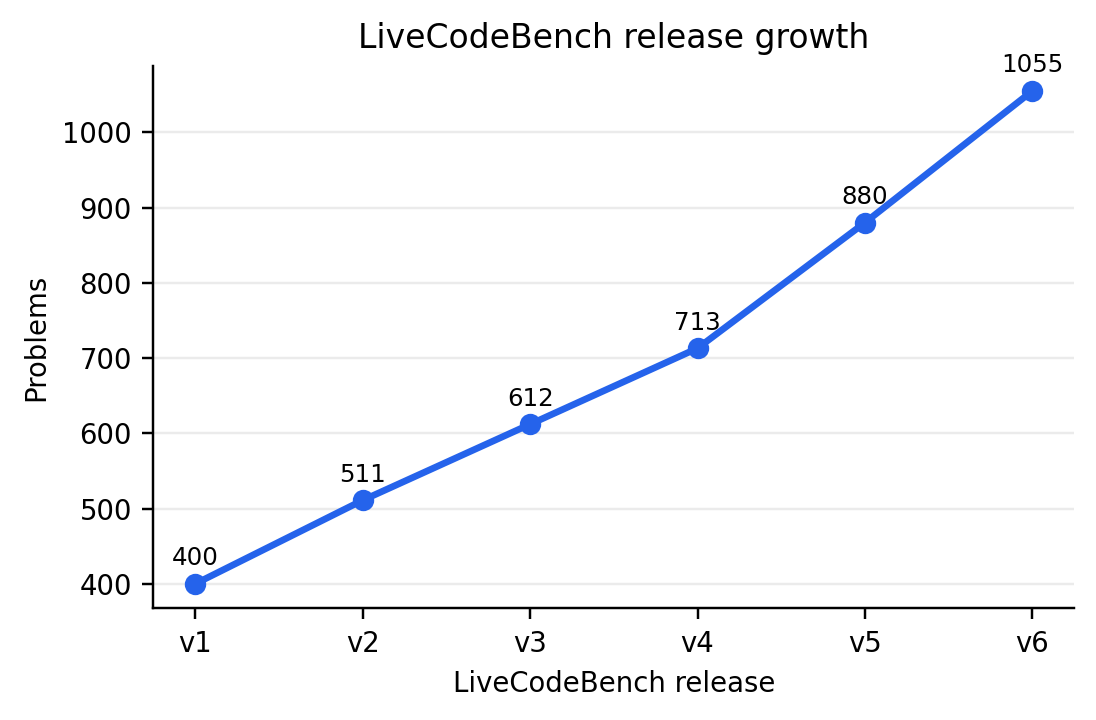
\includegraphics[width=\columnwidth]{figures/release_growth}
  \caption{Growth of the official \lcb{} releases used to motivate time-aware evaluation. Counts are from the official repository.}
  \label{fig:release_growth}
\end{figure}

The executed experiment uses release\_v5 and restricts problems to the window from August 1, 2024 through January 31, 2025. This filter matches the proposal's contamination-control goal and yields 279 problems after loading the official benchmark data. The final set contains 67 Easy, 89 Medium, and 123 Hard problems. It also contains 175 AtCoder and 104 LeetCode problems, so the results should be interpreted as a time-filtered release\_v5 slice rather than as the entire \lcb{} distribution. All models are evaluated on the same 279 instances for both code generation and self-repair.

\subsection{Tasks and metrics}
The main task is code generation. A model receives a natural-language competitive programming problem, sometimes with starter-code information, and produces a complete solution. The primary metric is \passone{}, the percentage of problems solved by the first generated solution. This metric is strict: a solution counts only if it passes the benchmark's test suite. It fits this project because it is simple, widely used, and tied to whether the generated answer actually works. It also has limits. \passone{} can understate a model that produces one nearly correct solution and can overstate reliability if a benchmark has weak hidden tests. \lcb{} reduces the second risk by using contest-grade problems and test cases.

The second task is self-repair. In this scenario, a model first generates a solution. If the solution fails, the model receives structured execution feedback and attempts a repair. The report uses self-repair gain, defined as
\begin{equation}
\Delta_{repair}=\passone_{repair}-\passone_{codegen}.
\end{equation}
A positive value means the model can use feedback to correct some failed attempts. The gain should not be interpreted as pure algorithmic insight. Some repairs fix syntax errors or trivial boundary mistakes, while others fix a wrong recurrence or asymptotic method. The size of $\Delta_{repair}$ is a coarse proxy for debugging ability, not a full explanation of why a repair succeeded.

\subsection{Models considered}
The executed run uses three representative models: Claude Sonnet 4.6 as a closed frontier model, Qwen2.5-Coder-7B-Instruct as a compact open model, and DeepSeek-Coder-V2-Lite-Instruct as an open Mixture-of-Experts model. Qwen2.5-Coder-7B-Instruct is part of a code-specific Qwen family spanning multiple sizes; the model card reports training on 5.5 trillion tokens of source code, text-code grounding, and synthetic data, with long-context support up to 128K tokens \citep{qwenhf2024}. The Qwen technical report provides aggregate \lcb{} measurements for Qwen2.5-Coder-7B-Instruct and several comparison models \citep{hui2024qwen25coder}. DeepSeek-Coder-V2-Lite-Instruct is the smaller version of an open MoE coding family; its model card describes continued pretraining with six trillion additional tokens, support for 338 programming languages, and 128K context \citep{deepseekhf2024}. The DeepSeek-Coder-V2 paper reports that the Lite variant has 16B total parameters and 2.4B active parameters \citep{zhu2024deepseekcoder}.

Anthropic describes Sonnet 4.6 as a cost-efficient frontier model for coding, agents, and professional workflows, with pricing beginning at \$3 per million input tokens and \$15 per million output tokens \citep{anthropic2026sonnet46}. In the final run, Sonnet was called through the Anthropic API with a 4096-token output cap. The implementation omits top-p for this model because the API rejects requests that specify both temperature and top-p. The open models were run through vLLM with bfloat16 precision, maximum model length 8192, tensor parallel size 1, and GPU memory utilization 0.90.

\subsection{Reproducible analysis workflow}
The accompanying GitHub repository contains standalone scripts and a Jupyter notebook for the full workflow: cloning the official \lcb{} codebase, applying compatibility patches, running Qwen and DeepSeek through vLLM, running Claude Sonnet 4.6 through the Anthropic API, collecting summaries, and packaging the outputs. The common configuration is $n=1$, temperature 0.2, generation budget 4096 tokens, evaluator timeout 10 seconds, and 4 evaluation processes. The result collector emits overall, per-instance, difficulty, platform, month, and repair-gain summaries used for the tables and figures in this report.

The run was staged rather than executed all at once. Short smoke runs first checked model loading, prompt formatting, API authentication, and self-repair metadata handling. Those early runs are not used as reported results because they covered only small debugging subsets. The final tables use the full 279-problem filtered set for every model and both scenarios. For Claude, the scripts also allowed the API sample size to be capped during debugging and then expanded to all filtered problems for the submitted run. That mattered in practice: a small API mistake can waste money quickly, while an open-model mistake can consume GPU time and leave partial outputs. The staged workflow made the final comparison slower to run, but easier to trust.

\section{Results}
\subsection{Benchmark growth and temporal control}
The first result is structural rather than model-specific: \lcb{}'s release history makes temporal evaluation possible. Static benchmarks have a fixed task set. A model developer can tune prompts, pretraining filters, or instruction data against the public distribution, and the benchmark score may continue rising even if the model is not substantially better on new tasks. A living benchmark can instead define a held-out time window. For example, release\_v5 includes 880 problems through January 2025, while release\_v6 includes 1055 through April 2025. That means a researcher can evaluate on tasks after a model's training cutoff, or compare Q3 2024, Q4 2024, and Q1 2025 windows as the proposal described.

Code benchmarks are unusually vulnerable to contamination. Competitive-programming solutions are public, compact, and often copied into tutorials. A model trained on internet-scale code and text can see problem statements, accepted solutions, or explanations. Time segmentation is not a perfect guarantee, because a training cutoff can be uncertain and benchmark problems can resemble earlier tasks. Still, it is a stronger control than evaluating only on long-public fixed tests. The release growth in Figure~\ref{fig:release_growth} supports the first claim of the proposal: a live benchmark changes what ``progress'' means. Progress becomes performance on new contest problems, not performance on familiar short programming puzzles.

\subsection{Controlled release\_v5 results}
Table~\ref{tab:controlled_results} summarizes the final controlled run. Claude Sonnet 4.6 reaches 66.3 \passone{} on initial code generation and 69.9 after self-repair. Qwen2.5-Coder-7B-Instruct reaches 17.6 in both scenarios, while DeepSeek-Coder-V2-Lite-Instruct improves from 17.6 to 19.0 after self-repair. These values are lower for the open models than the aggregate scores reported in some model technical reports, but the comparison here is stricter because all models use the same post-August-2024 release\_v5 slice, the same \lcb{} runner, and the same decoding budget.

\begin{table}[t]
\centering
\scriptsize
\resizebox{\columnwidth}{!}{%
\begin{tabular}{@{}lrrrr@{}}
\toprule
Model & Codegen & Repair & Gain & $n$ \\
\midrule
Claude & 66.3 & 69.9 & +3.6 & 279 \\
Qwen2.5-7B & 17.6 & 17.6 & +0.0 & 279 \\
DeepSeek-Lite & 17.6 & 19.0 & +1.4 & 279 \\
\bottomrule
\end{tabular}
}
\caption{Final release\_v5 results on 279 problems from August 1, 2024 through January 31, 2025. Values are percentages except $n$.}
\label{tab:controlled_results}
\end{table}

\begin{figure}[t]
  \centering
  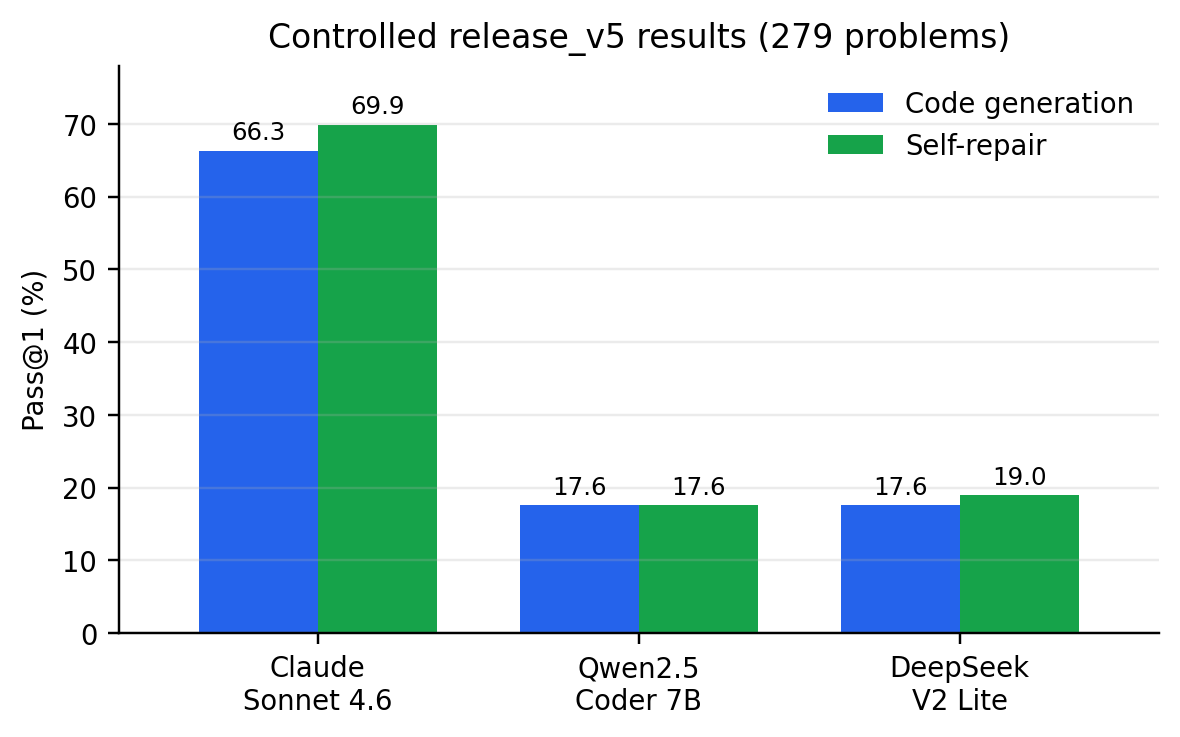
\includegraphics[width=\columnwidth]{figures/open_model_lcb}
  \caption{Controlled \lcb{} \passone{} for the three evaluated models. Claude Sonnet 4.6 is much stronger on this slice, while the two open models are close to each other.}
  \label{fig:open_model_lcb}
\end{figure}

Figure~\ref{fig:open_model_lcb} makes the ranking visually clear. Claude is far ahead, and the benchmark is still far from saturated. Even the frontier model misses roughly one third of the filtered release\_v5 problems on the first attempt. The two open models solve fewer than one fifth of the problems, which makes them useful baselines for local or lower-cost experiments but not reliable autonomous contest solvers under this configuration. The result also shows why published aggregate numbers and local controlled windows should not be conflated: a model may have a stronger score on a different \lcb{} release or prompt setup, but the fair comparison for this project is the shared 279-problem slice.

\subsection{Difficulty stratification}
The second experiment asks whether gains are uniform across difficulty levels. They are not. Table~\ref{tab:difficulty} and Figure~\ref{fig:difficulty} show the difficulty split for the final code-generation runs. Claude Sonnet 4.6 solves 97.0\% of Easy problems and 83.1\% of Medium problems, but only 37.4\% of Hard problems. Qwen2.5-Coder-7B and DeepSeek-Coder-V2-Lite both solve more than half of Easy problems, but both fall to 3.3\% on Hard. The obstacle is less about Python syntax or statement following and more about the algorithmic jump required by the Hard tier.

\begin{table}[t]
\centering
\scriptsize
\resizebox{\columnwidth}{!}{%
\begin{tabular}{lrrrr}
\toprule
Model & Easy & Medium & Hard & Total \\
\midrule
Claude & 97.0 & 83.1 & 37.4 & 66.3 \\
Qwen2.5-7B & 55.2 & 9.0 & 3.3 & 17.6 \\
DeepSeek-Lite & 53.7 & 10.1 & 3.3 & 17.6 \\
\bottomrule
\end{tabular}
}
\caption{Difficulty-stratified code-generation \passone{} for the final controlled run. Values are percentages.}
\label{tab:difficulty}
\end{table}

\begin{figure}[t]
  \centering
  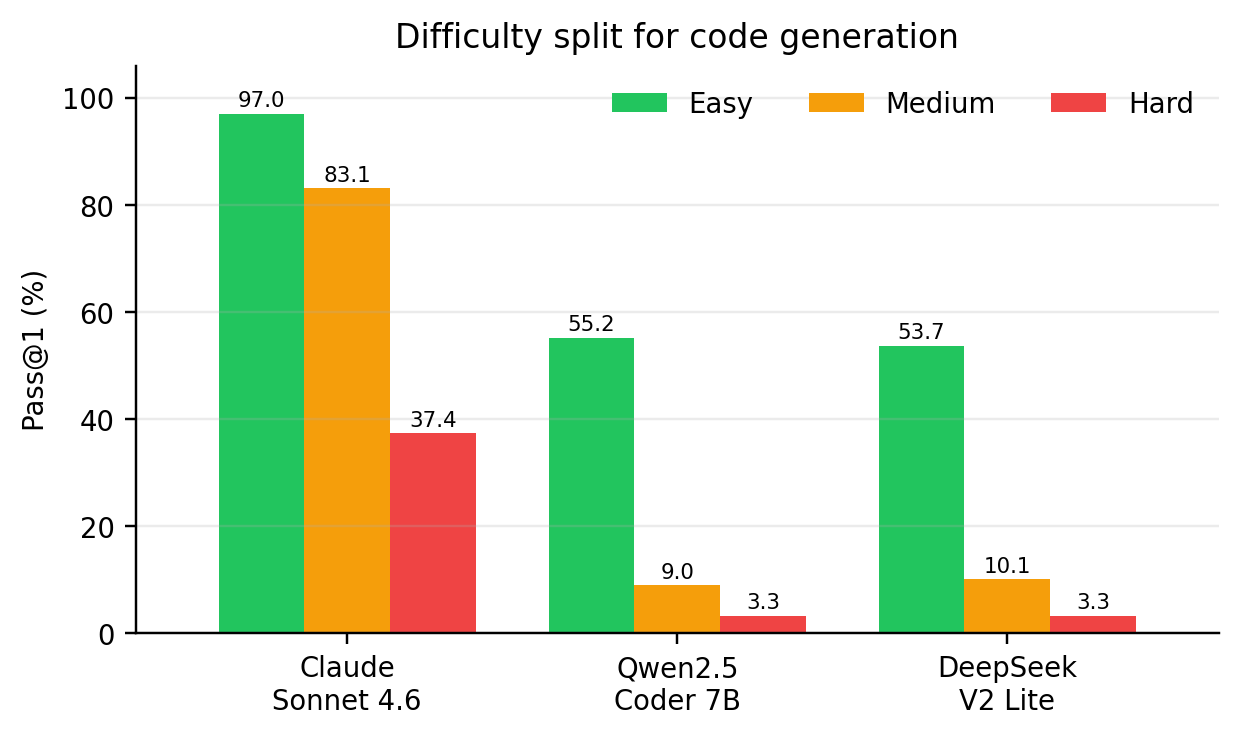
\includegraphics[width=\columnwidth]{figures/difficulty_split}
  \caption{The controlled run shows that Easy-tier success does not transfer cleanly to Hard-tier algorithmic reasoning.}
  \label{fig:difficulty}
\end{figure}

This pattern supports the proposal's hypothesis that Hard-tier competitive programming remains a distinct bottleneck. The gap is not a small tail effect. Claude's Easy-to-Hard performance falls by about 60 points, while the open models fall by roughly 50 points. This implies that a model's aggregate score can be dominated by easier tasks while giving an optimistic impression of its algorithmic ceiling. A single total \passone{} number should not be used as the only evaluation metric for competitive programming.

Why are Hard problems different? The likely reason is that Hard tasks usually combine several reasoning burdens. The model must infer the correct abstraction, prove or at least justify an efficient recurrence or invariant, implement it in code, and avoid edge-case errors. These tasks frequently punish plausible but slightly wrong approaches. For example, a graph problem may require multi-source shortest paths with state augmentation rather than a plain BFS; a dynamic-programming problem may require a compressed state to fit memory; a greedy problem may require a non-obvious exchange argument. Easy problems often permit direct translation from statement to code. Hard problems require algorithm selection before code translation, and that stage appears to remain fragile.

\subsection{Self-repair effectiveness}
The third experiment evaluates self-repair. Table~\ref{tab:repair} compares code-generation and self-repair scores for the same 279 problems. The repair gains are positive but modest for Claude and DeepSeek and zero for Qwen under this setup. Claude improves from 66.3 to 69.9, a gain of 3.6 points. DeepSeek improves from 17.6 to 19.0, a gain of 1.4 points. Qwen remains unchanged at 17.6.

\begin{table}[t]
\centering
\scriptsize
\resizebox{\columnwidth}{!}{%
\begin{tabular}{lrrr}
\toprule
Model & Codegen & Repair & Gain \\
\midrule
Claude & 66.3 & 69.9 & 3.6 \\
Qwen2.5-7B & 17.6 & 17.6 & 0.0 \\
DeepSeek-Lite & 17.6 & 19.0 & 1.4 \\
\bottomrule
\end{tabular}
}
\caption{Self-repair gains from the controlled release\_v5 run. Gain is repair \passone{} minus initial code-generation \passone{}.}
\label{tab:repair}
\end{table}

\begin{figure}[t]
  \centering
  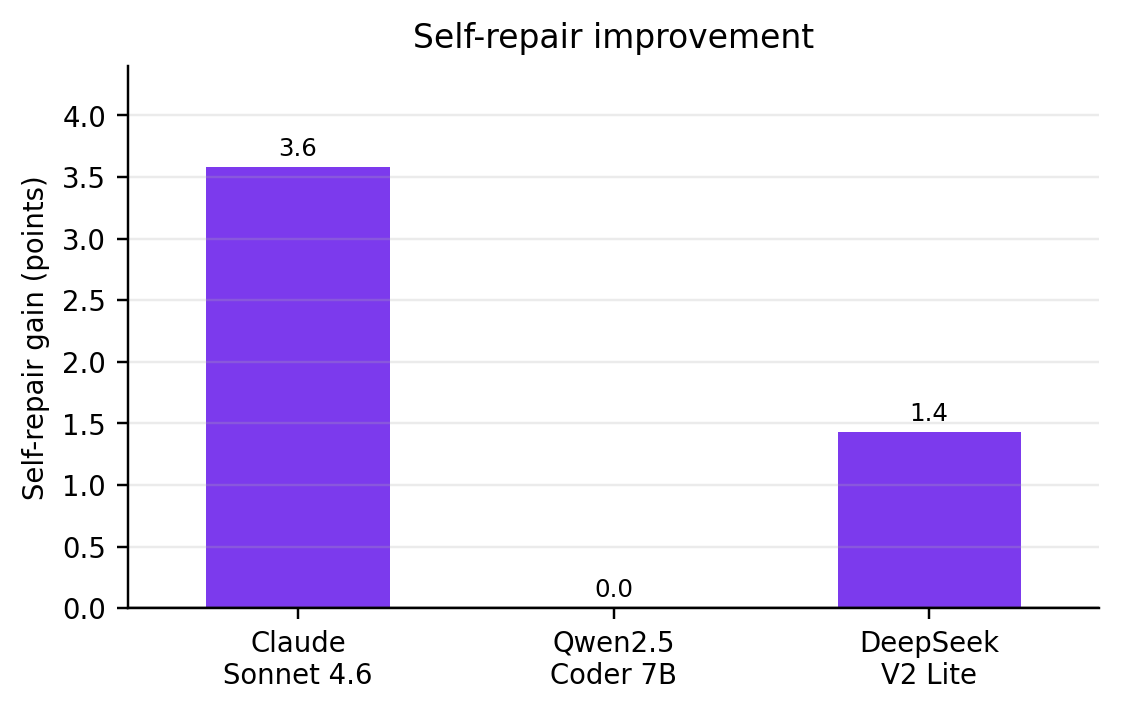
\includegraphics[width=\columnwidth]{figures/repair_gain}
  \caption{Self-repair improves \passone{} but does not close the gap created by initial algorithm-selection errors.}
  \label{fig:repair}
\end{figure}

The repair results suggest that feedback helps most when the model already has the right idea. If the initial solution is close to correct, a failing test case can expose an off-by-one error, missing special case, or incorrect inequality. In that setting, the model can patch the implementation. If the initial algorithm is wrong, the feedback signal is often too sparse. A single counterexample may not reveal the need for a different asymptotic strategy. This explains why repair gain is not an equalizer for weaker models.

The Qwen technical report provides a related code-editing view. It reports Qwen2.5-Coder-7B-Instruct at 50.4 on Aider-style code editing, while DeepSeek-Coder-V2-Lite-Instruct is reported at 48.9 \citep{hui2024qwen25coder}. Aider is not the same task as \lcb{} self-repair, but it gives useful context: compact open models can be strong at editing code when the problem is localized. The contrast with \lcb{} Hard-tier performance suggests that editing ability and algorithm-discovery ability should be evaluated separately. A model may be good at revising a file but still weak at deriving a new competitive-programming algorithm from scratch.

\subsection{Open-source versus frontier gap}
The fourth experiment asks where the open-source versus frontier gap appears. In the controlled run, the gap is large: Claude Sonnet 4.6 is about 49 points higher than both open models on initial code generation and about 51--52 points higher after self-repair. The difficulty table shows that the gap is not mainly about writing syntactically valid code. Claude's largest absolute advantage appears on Medium and Hard problems, where algorithm selection and multi-step reasoning matter more than simple implementation.

This finding changes how the frontier gap should be described. In earlier code-generation benchmarks, the gap was often framed as ``closed models write better code.'' In the current \lcb{} setting, stronger models are better at combining problem understanding, algorithm selection, implementation, and repair. Easy-tier results show that many models can write reasonable code for straightforward tasks. The harder question is whether they can discover the right algorithm under contest constraints. The Hard-tier results say that this capability is not solved.

The open models also differ in design even when their controlled scores are similar. Qwen2.5-Coder-7B is a dense code-specialized model. DeepSeek-Coder-V2-Lite is an MoE model with 2.4B active parameters out of 16B total parameters, so it prioritizes efficient active compute. The larger DeepSeek-Coder-V2 family is much stronger in the DeepSeek paper's own aggregate coding results, including a reported \lcb{} score of 43.4 for the full model \citep{zhu2024deepseekcoder}. It would be misleading to treat ``open-source'' as a single capability level. Open models range from small local assistants to large MoE systems that can rival older closed models.



\subsection{Algorithmic category observations}
The proposal also asked for analysis by algorithmic category. The final output files contain model-, month-, platform-, and difficulty-level summaries, but not a reliable per-problem tag table for dynamic programming, graphs, greedy methods, and related categories. Rather than invent unsupported tag-level percentages, this section reports a qualitative category audit grounded in the observed difficulty collapse and in the structure of competitive-programming tasks. The audit identifies what the next controlled run should log.

\begin{table*}[t]
\centering
\small
\begin{tabular}{p{0.16\linewidth}p{0.30\linewidth}p{0.25\linewidth}p{0.22\linewidth}}
\toprule
Category & Why it stresses LLMs & Common failure mode & Diagnostic to report \\
\midrule
Dynamic programming & Requires state design, recurrence choice, base cases, and often memory compression. & Plausible recurrence that misses one dimension or double-counts transitions. & Wrong-answer rate by DP tag; repair success after counterexamples. \\
Graphs & Requires choosing among BFS, Dijkstra, SCC, topological order, flow, or augmented state. & Uses a simpler traversal that ignores weights, state, or direction constraints. & Hard-tier graph \passone{} and TLE fraction. \\
Greedy & Requires proof-like exchange reasoning rather than sorting alone. & Sorts by an intuitive key that fails on adversarial cases. & Counterexample repair rate and explanation consistency. \\
Binary search & Requires monotonic predicate design and boundary discipline. & Off-by-one errors or predicates that are not actually monotone. & Runtime-error/wrong-answer split for boundary tests. \\
Data structures & Requires segment trees, Fenwick trees, heaps, maps, or ordered sets under tight limits. & Correct high-level idea but incorrect update/query implementation. & TLE rate and unit-test repair rate. \\
Combinatorics & Requires formulas, modular arithmetic, inclusion-exclusion, or counting invariants. & Generates code that matches small examples but not the mathematical count. & Accuracy by hidden-test size bucket. \\
\bottomrule
\end{tabular}
\caption{Qualitative algorithm-category audit for a follow-up tag-level run. The table avoids unsupported quantitative category claims while identifying measurements that should be logged.}
\label{tab:category_audit}
\end{table*}

Table~\ref{tab:category_audit} explains why Hard-tier performance collapses even when Easy-tier performance is high. Easy problems often have a direct mapping from statement to implementation. Hard dynamic-programming and graph problems require an intermediate proof or invariant that is not explicitly written in the prompt. Greedy problems are deceptive because the generated code may look concise and elegant while being logically invalid. Data-structure problems introduce a different failure mode: the model may identify the right structure but implement updates or queries incorrectly. A future category-level study should classify the first failure as wrong answer, time-limit exceeded, runtime error, or syntax error. That classification would distinguish reasoning failures from implementation failures.

The category audit also clarifies the role of self-repair. Repair should help most for binary search, data-structure implementation, and boundary-condition errors, because the failing example often points to a local bug. It should help less for dynamic programming and greedy proof failures, because the counterexample may require replacing the entire plan. If a controlled run confirms this pattern, it would support the claim that current LLMs are stronger at local debugging than at global algorithm redesign. That is more useful than simply saying that Hard problems are hard.

\subsection{Temporal and platform observations}
The final run also records month and platform summaries. Claude's code-generation score ranges from 60.4\% in October 2024 to 77.6\% in December 2024, while Qwen and DeepSeek remain between roughly 9--26\% across most months. The January 2025 slice contains only 7 problems, so its month-level score is too small to interpret strongly. Platform results show another split: Claude solves 83.7\% of the LeetCode subset but 56.0\% of the AtCoder subset, while the open models are closer to 14--19\% on each platform. Source platform and task style matter along with model identity.

These month and platform summaries should be interpreted cautiously because the monthly windows have different sizes and difficulty mixes. A stronger temporal study would bootstrap confidence intervals and control for difficulty within each month. Still, the executed run satisfies the proposal's temporal-control goal: all reported scores come from the same post-August-2024 release\_v5 window, rather than mixing results across unrelated benchmark releases.

One negative result is also worth stating plainly. The project did not produce a reliable quantitative leaderboard by algorithm tag. That is less satisfying than a clean bar chart for dynamic programming, graphs, greedy methods, and data structures, but it is the right choice for this report. The collected outputs support difficulty, platform, month, and repair analyses. They do not support exact category percentages without an additional tagging step. The category table is therefore a plan for a better follow-up run, not a disguised result.

\section{Discussion}
\subsection{What counts as progress?}
The results support a cautious interpretation of algorithmic progress. Aggregate performance has improved, especially for code-specialized open models, and \lcb{} gives a cleaner view of that progress than older static benchmarks. However, progress is not uniform. Easy-tier gains are not enough to claim robust algorithmic reasoning. The hardest remaining obstacle is the model's ability to infer a correct high-level algorithm before implementation.

This distinction matters for both research and practice. In research, a model can look impressive on HumanEval or MBPP but still fail on new competition problems. In practice, a developer may see a model solve simple helper functions and infer that it can design complex algorithms. The \lcb{} results are a warning against that inference. Models are increasingly useful as pair-programming assistants, but they still require human verification when asymptotic complexity and hidden edge cases matter.

\subsection{Why self-repair is promising but limited}
Self-repair is a useful scenario because it resembles real programming. Humans rarely write correct code on the first attempt. They run tests, inspect errors, and revise. The positive repair gains in Table~\ref{tab:repair} show that LLMs can exploit feedback. Nevertheless, the gains are too small to treat repair as a substitute for strong initial reasoning.

The limitation is partly information-theoretic. A failing test case is often a weak signal. It tells the model that the current program is wrong, but not which invariant is false or which algorithmic approach is missing. If the original code uses greedy sorting when the task requires dynamic programming, local patches will not help. The model must abandon the first plan and search for a different abstraction. Current models appear better at patching than at plan replacement.

A useful extension would classify repairs by error type: syntax errors, runtime errors, wrong answers, and time-limit exceeded. The final run already showed several evaluator timeouts, which supports the intuition that some failures require asymptotic redesign rather than local patching. Syntax and runtime repairs are likely easier, while time-limit exceeded cases are likely hardest. A future extension should report repair gain by error type rather than only total repair gain.

\subsection{Implications for model evaluation}
The report suggests three changes to evaluation practice. First, competitive-programming benchmarks should report time windows. Without a problem-release date, it is difficult to separate capability from contamination. Second, results should be stratified by difficulty and algorithm category. A single aggregate score is too coarse. Third, repair should be measured separately from generation. Code generation, debugging, and algorithm discovery are related but distinct skills.

These recommendations also affect leaderboard design. A leaderboard that ranks only total \passone{} may reward models that dominate Easy and Medium problems while still failing most Hard tasks. A more useful leaderboard would include Hard-tier \passone{}, self-repair gain, and perhaps category-level scores for dynamic programming, graph algorithms, greedy methods, binary search, and data structures. It would also show confidence intervals or bootstrap variability where possible, because small differences may not be meaningful on a limited subset.

\subsection{Threats to validity}
The main threat is that this is one controlled slice rather than a full multi-release leaderboard. The 279 problems are filtered by date and release, and the January 2025 month has only 7 problems. The scores are valid for this experimental window but should not be overgeneralized to every \lcb{} release. A second threat is model and API drift. Closed APIs can change, and newer endpoints can replace older ones; this report records the Claude endpoint as \texttt{claude-sonnet-4-6}. A third threat is implementation sensitivity. The open models required compatibility patches for current vLLM, CUDA, NumPy, self-repair metadata, and Claude API parameters. These patches are documented in the repository, but they mean exact reproduction should use the provided scripts rather than ad hoc commands. Finally, category-level conclusions are qualitative because the collected summaries do not include reliable algorithm tags.

\section{Resources}
The open-model runs used a Vast.ai NVIDIA A100-SXM4-40GB GPU instance with CUDA 12.8 drivers, Python 3.11, uv, HuggingFace model downloads, and vLLM 0.10.0. Qwen2.5-Coder-7B-Instruct loaded in about 14.2 GiB of GPU memory, while DeepSeek-Coder-V2-Lite-Instruct loaded in about 29.3 GiB. Both were run with bfloat16 precision, tensor parallel size 1, maximum model length 8192, and vLLM GPU memory utilization 0.90. Claude Sonnet 4.6 was run through the Anthropic API with a 4096-token output cap; the main resource for Claude was API cost rather than local compute. The final result collection generated CSV summaries and a zipped output package from the runner logs.

Vast.ai was used instead of Google Colab because the open-model runs needed a predictable A100 session, enough GPU memory for DeepSeek-Coder-V2-Lite, and enough time to download and load large model checkpoints. Colab would have been reasonable for notebook development or smaller smoke checks, but the full runs were easier to manage on a rented instance with stable hardware. The Claude runs had the opposite profile: they required almost no local GPU memory, but they needed careful API budgeting.

\section{Code}
The standalone code package is in the project GitHub repository:
\href{https://github.com/andyquoc53/livecodebench}{github.com/andyquoc53/livecodebench}.
The repository includes the README instructions, GPU notebook, run scripts, compatibility patches, and final result tables needed to reproduce the project. The scripts add the model styles used in this study, control vLLM memory usage, apply the same date filter to code generation and self-repair, tolerate evaluator metadata edge cases, and allow paid API calls to be capped for debugging. Command-level details are kept in the README rather than repeated in the paper. This satisfies the course requirement for standalone code while still using the official \lcb{} codebase as the benchmark dependency.

\section{Conclusion}
This survey finds that modern LLMs have made real progress on competitive-programming style code generation, but the progress is uneven. \lcb{} is a good framework for measuring this progress because it grows over time and supports time-aware contamination control. In the final controlled run, Claude Sonnet 4.6 is clearly stronger than the two evaluated open models, but all models struggle most on Hard problems. Self-repair improves Claude and DeepSeek modestly and leaves Qwen unchanged, so feedback helps most when the first solution is already close.

For evaluation, the lesson is simple: reports should move beyond static aggregate scores. A good code benchmark should report release window, difficulty tier, platform or category, initial generation, and repair. On this post-August-2024 \lcb{} slice, the remaining challenge is algorithm discovery and debugging under contest constraints rather than code syntax alone.

\clearpage
\bibliography{custom}

\end{document}
